\begin{savequote}[75mm]
  There is no unique picture of reality.
  \qauthor{Stephen Hawking}
\end{savequote}

\chapter{High Energy Physics}

The idea of atoms - building blocks of nature stretches back as far as ancient Greece, to Leucippus and Democritus \cite{10.3138/9781442671102}, and prevailed through the ages until the beginning of the 20th century, when it was solidified. In 1897 J.J.Thompson discovered an electron using a cathode ray and noticed its negative charge \cite{thomson1901bodies}.
Later in 1911, Rutherford discovered the nucleus using the gold foil scattering experiment \cite{doi:10.1080/14786440508637080}.
Shortly after that, in 1932, the model of the nucleus containing neutron and proton was developed \cite{Iwanenko1932TheNH, 1932ZPhy...77....1H}.
These events, along with the development of quantum mechanics, laid a foundation for the development of modern physics.
The deeper we wanted to look inside the matter, and the deeper it  was probed by the physics, the more different particles were found.
This ``particle zoo'' was later explained with Quantum Field Theory and a small number of fundamental particles.
Those fundamental particles and the rules that guide their interactions are combined into Standard Model - the best theory developed by our civilisation so far.
This chapter serves as an introduction to the theoretical concepts fundamental to understanding the purpose of the LHCb detector and the research presented in this thesis.
The Sections \ref{sec:tree-ckm} and \ref{sec:lepton-uni} contain two examplary directions of research done by the LHCb collaboration (not contributed by the author).

\section{Standard Model}

\begin{figure}
  \centering
  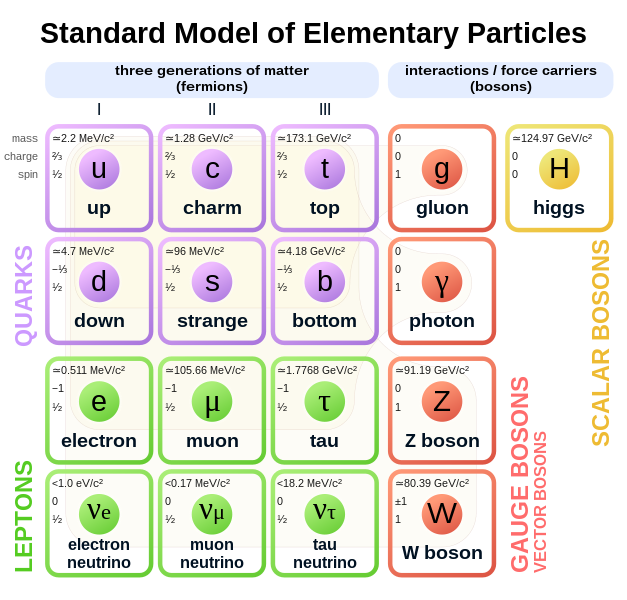
\includegraphics[width=0.7\linewidth]{figures/chapter1/Standard_Model_of_Elementary_Particles.svg.png}
  \caption[caption for LOF]{Standard model of Elementary Particles \footnotemark}
  \label{fig:standard_model}
\end{figure}



Standard model (schematically depicted in Fig. \ref{fig:standard_model}) consists of two types of particles: bosons and fermions. Bosons are responsible for the interactions, and fermions constitute matter (Neutrons, Protons, Atoms).
Furtherly, the fermions consist of three generations of leptons and quarks.
There are six quarks: up, down, charm, strange, top, and beauty. Two up quarks and one down quark combine into a proton, and one up quark and two down quarks combine into a neutron.
The combinations of quarks create the particle zoo. In fact, the quarks have never been observed as free particles, which is explained by the colour confinement.
The most popular combinations of quarks consist of two (mesons - quark and antiquark pair) and three quarks, with other combinations like pentaquarks much less probable but still possible.
Half of the fermions are leptons and have been observed as free particles, unlike quarks. The three charged leptons are electron, muon, and tau; all have an electric charge of -1.
The other three are three flavours of neutrinos: electron neutrino, muon neutrino, tau neutrino.
The neutrinos are charge-less and have a negligibly small mass. Due to that, they are very elusive and hard to study.
\footnotetext{ Source \url{https://en.wikipedia.org/wiki/File:Standard_Model_of_Elementary_Particles.svg}}
The Bosons are the particles that carry the interactions. There are twelve gauge vector bosons and one scalar boson.
The gauge bosons consist of a photon, eight gluons, two charged W bosons and one neutral Z boson.
The photon is a carrier of electromagnetic force and is massless and chargeless.
The strong nuclear force is propagated by gluons, which, similarly to the photon, are mass and charge-less, but unlike a photon, they can't exist as a free particle and carry the colour charge.
The W and Z bosons are responsible for the weak nuclear force.
Their exchange can change the flavour of the interacting quark or lepton.
The one scalar boson - the Higgs boson, is famously the newest addition to Standard Model.
The Higgs boson is responsible for attributing mass to W and Z bosons and fermions.

Additionally to the particles described above, each fermion has a corresponding anti-matter partner. In case of bosons we assume, according to Standard Model, that they are their own antiparicles (apart from W bosons).

The Large Hadron Collider and its accompanying detectors were created to study various implications of Standard Model. A few of the LHCb experiment's primary goals are presented below.


% \section{proton proton collisions}
\section{CP symmetry violation}
One of the cosmology's greatest mysteries is the severe inequality between matter and anti-matter in the observable universe. The simple assumption would be that there should be equal amounts of matter and anti-matter if the rules of physics are the same for matter and anti-matter.
The most probable cause for such a state is that soon after the Big Bang, the C-, P- and CP-symmetries (\textbf{C} for the charge parity operation, \textbf{P} for the space parity operation) were broken what led to creation of significantly more matter than antimatter.
The CP violation study is conducted to explain this phenomenon.

The parity inversion operator, \textbf{P}, can be defined as a mirror inversion:

$$
P\psi(r) = \psi(-r)
$$

There used to be a belief that physics is invariant under this operation, which was verified in strong and electromagnetic interactions but was not verified in weak interactions \cite{PhysRev.104.254}.
This led to experiments showing that some of the reactions in beta decay do not occur as frequently as their mirror image.
The next idea was that although parity itself may not be conserved, the conjugation of the charge parity operator combined with the spatial parity one constitute an exact symmetry.
The charge parity operator can be defined as an operator which changes a particle into its anti-particle by changing the sign of its additive quantum numbers (e.g., the charge):
$$
C \, |\psi\rangle = | \bar{\psi}\rangle.
$$

The combined $CP$ symmetry is also broken \cite{PhysRevLett.13.138} in weak interactions. The LHCb reported a $CP$ violation in B meson \cite{PhysRevLett.110.221601} and charm decays \cite{PhysRevLett.122.211803}. The beauty decays can have the CP-asymmetry at the level of 80\%.

In the search for the invariant law of symmetry, an additional combination of $CPT$ symmetry ($T$ is the time-reversal operator) was proposed, which seems to be conserved in all known processes in Standard Model.

Although the studies have shown that there exist symmetry breaking processes in weak interactions of the quark sector, they do not explain the imbalance in matter and anti-matter in the universe.
An additional search for symmetry breaking in the lepton sector is also undergoing.


\section{Tree-level determination of the unitarity triangle angle γ - CKM matrix}
\label{sec:tree-ckm}

The CKM (Cabibo-Kobayashi-Maskawa) matrix elements describe the strength of the flavour change in weak interactions. I.e. $V_{ud}$ is the probability of the down quark transforming into an up quark.
$$
\begin{bmatrix}  d'  \\  s'  \\  b'  \end{bmatrix} = \begin{bmatrix} V_\mathrm{ud} & V_\mathrm{us} & V_\mathrm{ub} \\ V_\mathrm{cd} & V_\mathrm{cs} & V_\mathrm{cb} \\ V_\mathrm{td} & V_\mathrm{ts} & V_\mathrm{tb} \end{bmatrix} \begin{bmatrix}  d  \\  s  \\  b  \end{bmatrix}
$$

The most recent approximation of the CKM matrix values \cite{10.1093/ptep/ptaa104}, is as follows:

$$
\begin{bmatrix}
|V_{ud}| & |V_{us}| & |V_{ub}| \\
|V_{cd}| & |V_{cs}| & |V_{cb}| \\
|V_{td}| & |V_{ts}| & |V_{tb}|
\end{bmatrix} = \begin{bmatrix}
0.97370 \pm 0.00014 & 0.2245 \pm 0.0008 & 0.00382 \pm 0.00024 \\
0.221 \pm 0.004 & 0.987 \pm 0.011 & 0.0410 \pm 0.0014 \\
0.0080 \pm 0.0003 & 0.0388 \pm 0.0011  & 1.013 \pm 0.030
\end{bmatrix}.
$$


The CKM matrix can be understood as a rotation matrix in 3D (SU(3)) and, therefore, can be parametrised by independent angles.
It is helpful to use it with Wolfenstein parametrisation \cite{PhysRevLett.51.1945}, which allows parametrising the matrix in four independent values $\lambda$, $A$, $\rho$ , and $\nu$.

Such parametrisation allows for representation of the unitarity condition of the CKM  $V_{ud}V*_{ub} + V_{cd}V*_{cb}+ * V_{td}V*_{tb} = 0$ as a triangle:


\begin{figure}
  \centering
  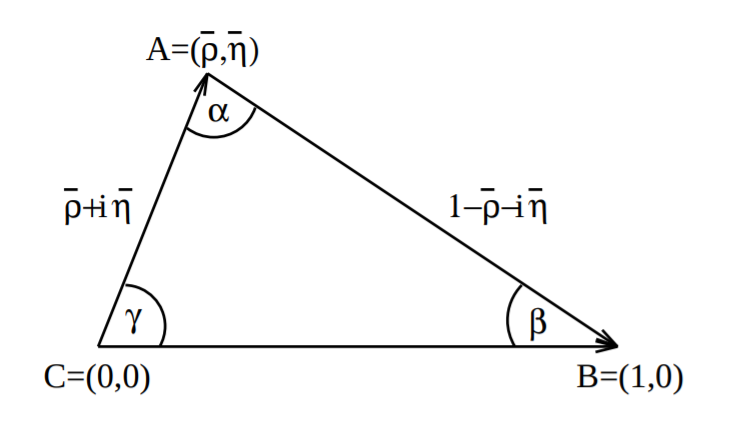
\includegraphics[width=0.6\linewidth]{figures/chapter1/UnitaryTriangle.png}
  \caption{A unitary triangle (source: \cite{buras2002unitarity})}
  \label{fig:unitary_triangle}
\end{figure}

Studies of various processes, mainly tree-level and loop processes, allow for calculating the constraints on the value of the $\gamma$ angle in the unitary triangle.


\begin{figure}[H]
\centering
\begin{subfigure}[b]{0.85\textwidth}
    \centering
    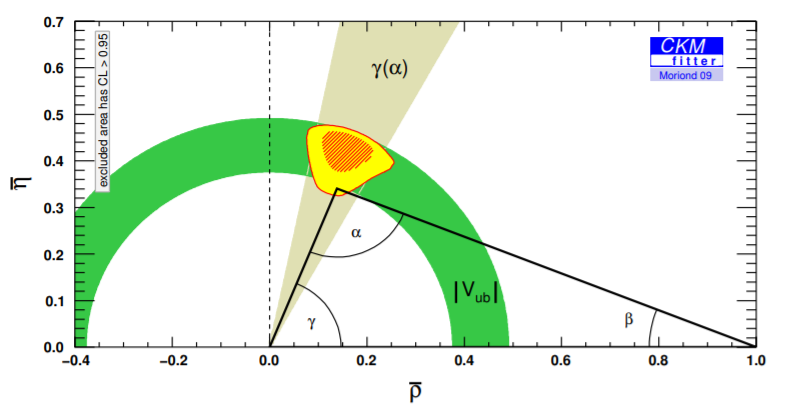
\includegraphics[width=\linewidth]{figures/chapter1/lhcb_goals_a.png}
\caption{}
   \label{plot:plot_triangle_a}
  \end{subfigure}
\begin{subfigure}[b]{0.85\textwidth}
    \centering
    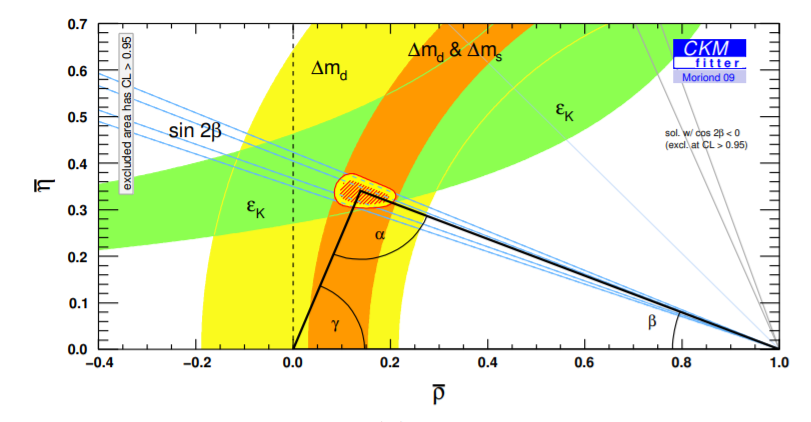
\includegraphics[width=\linewidth]{figures/chapter1/lhcb_goals_b.png}
\caption{Target (Y)}
   \label{plot:plot_triangle_b}
  \end{subfigure}
  \caption[Triangle constraints]{Constraints on the Unitarity Triangle from (a) tree and (b) loop processes, from 2009.}
    \label{plot:both_triangles}
\end{figure}

As can be seen in the \ref{plot:both_triangles}, the constraints on the tree-level before the LHC data taking periods \cite{thelhcbcollaboration2010roadmap} Run 1 and Run 2 studies were much broader than for the loop processes, which established the need for research in this direction.
The angle calculated by the LHCb for the tree-level decays as of 2020 is $γ = (67 \pm 4)^{\circ}$ \cite{LHCb-CONF-2020-003}.
The further studies in this area (difference between the tree-level and loop dominated processes) may hint new physics beyond standard model \cite{Krupa:2314451}.


\section{Test for the lepton universality.}
\label{sec:lepton-uni}

\begin{figure}
\begin{subfigure}[t]{0.5\textwidth}
  \centering
  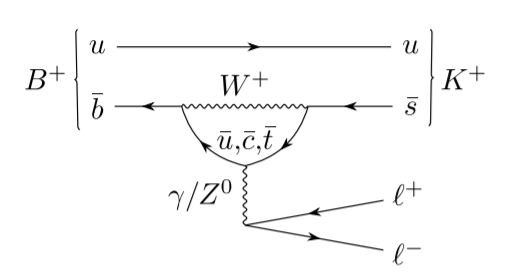
\includegraphics[width=\linewidth]{figures/chapter1/BKLL.png}
  \caption{A decay of $B^{+}$ into kaon and two leptons.}
\end{subfigure}
\begin{subfigure}[t]{0.5\textwidth}
  \centering
  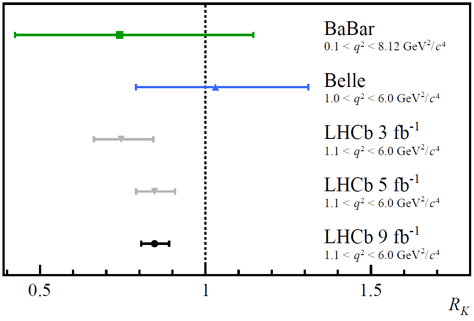
\includegraphics[width=\linewidth]{figures/chapter1/RK2021_s.png}
  \caption{Experimental results of the $R_{k}$ ration calculation.}
\end{subfigure}
 \caption[Experiments]{}
  \label{fig:bkll}
\end{figure}

The coupling of the leptons to the weak gauge bosons is expected to be identical. This is one of the consequences of the Standard Model.
This means that there should be similar decay ratios except for the different masses of the leptons.

The Lhcb collaboration tested this assumption using a $B^{+} \rightarrow  K^{+}\ell \ell $ decay.

As can be seen in the \ref{fig:bkll} process includes a change of the meson $B^{+}$ into kaon by weak force and change of $\bar{b}$ int $\bar{s}$.
The assumption coming from the Standard Model is that the ratios of electrons and muons produced in this process (leptons) should be close to 1. This ratio is called $R_{K}$ and is calculated as $R_{K} = BR(B^{+}\rightarrow K^{+}\mu^{+}\mu^{-})/BR(B^{+}\rightarrow e^{+}e^{-})$


The result of the studies at LHCb is $0.846^{+0.044}_{-0.041}$ \cite{lhcbcollaboration2021test} which is 3.1 standard deviations away from the Standard Model prediction, which hints at the breaking of the lepton universality.
If this result were confirmed with greater confidence, it would suggest new physics beyond the standard model.
%th
